\documentclass[a4]{scrartcl}

% \usepackage[ngerman]{babel}
\usepackage[utf8]{inputenc}
\usepackage{mathtools}
\usepackage{amsmath}
\usepackage{amssymb}
\usepackage{geometry}
\usepackage{scrlayer-scrpage}
\usepackage{float}
\usepackage{xcolor}
\pagestyle{scrheadings}
\clearscrheadfoot

\usepackage[backend=biber, maxbibnames=99]{biblatex}
\addbibresource{references.bib}

\setlength{\parindent}{0cm}


\geometry{
  paper=a4paper, % Change to letterpaper for US letter
  top=2cm, % Top margin
  bottom=1.5cm, % Bottom margin
  left=2cm, % Left margin
  right=3cm, % Right margin
}

\ohead{\\
Pina Kolling\\
piko0011}

\usepackage[framemethod=TikZ]{mdframed}

% Style %
\mdfdefinestyle{enviStyle}{
   innertopmargin = 10pt,
  linewidth      = 1pt,
  frametitlerule = true,
  roundcorner    = 2pt%
}


\newenvironment{CountingDefinition}[2][]{%
   \ifstrempty{#1}%
   {\mdfsetup{%
      frametitle={{\strut ~}}}
   }%
   {\mdfsetup{%
      frametitle={{\strut ~#1}}}%
   }%
   \mdfsetup{
      nobreak                   = true,
     linecolor                 = gray,
    frametitlebackgroundcolor = gray!50,
    style                     = enviStyle
   }
   \begin{mdframed}[]\relax%
   \label{#2}}{\end{mdframed}}

\begin{document}

\section*{Summary: Lecture 7}

Summary for the chapters \textit{9.1} and \textit{9.2}. \cite{book, CC}

\subsection*{NP-Completeness}

\begin{CountingDefinition}[NP]{def:validLabelPlacement}
Class of lanugages decided by nonderteministic Turing machines in polynomial time.

Most problems are in NP.
\end{CountingDefinition}

\textbf{NP-completeness:}
\begin{itemize}
\item easiest problems among those we do not know how to solve efficiently
\item if P$\neq$NP can be proven: exact border of efficient solvability is found
\item best bet for proving P$=$NP: show that some NP-complete problem is $P$
\item Until then, the NP-complete problems are the least likely ones in NP to be efficiently solved
\item Where is the line between P and NP?
\end{itemize}



\begin{CountingDefinition}[Lanugage $L$]{def:validLabelPlacement}
$L= \{ x: (x,y) \in R \textit{ for some } y \}$ \ 
\\
$L$ gets an input $x$ and finds a $y$ with $((x,y) \in R$ and the relation $R \subseteq \Sigma^* \times \Sigma^*$.
\end{CountingDefinition}


\textbf{Polynomially decidable:}
\begin{itemize}
\item $R$ is polynomially decidable if there is da deterministic Turing machine deciding the language $L$ in polynomial time
\item then the relation $R$ (not the language $L$) is polynomially decidable
\end{itemize}

\textbf{Polynomially balanced:}
\begin{itemize}
\item $R$ is polynomially balanced if $(x,y) \in R$ implies $|y| \leq |x|^k$ for some $k \geq 1$ \\
$\rightarrow$ length of the second component is bounded by a polynomial in the length of the first
\item then the relation $R$ (not the language $L$) is polynomially balanced
\end{itemize}

\begin{CountingDefinition}[NP]{def:validLabelPlacement}
The language $L \subseteq \Sigma^*$ is in NP only if there is a polynomially decidable and polynomially balanced relation $R$ such that  $L= \{ x: (x,y) \in R \textit{ for some } y \}$.
\end{CountingDefinition}

For example: Is there a satisfying assignment ($y$) for a formular ($x$)?


\ \\
\textbf{Proof idea:}
\begin{itemize}
\item
\end{itemize}

\ \\ \ \\

\color{red} TODO \\
proof \\
\color{black}


\subsection*{Succinct certificate (for NP-complete problems)}

\begin{itemize}
\item \textit{yes} instance of $x$ has a polynomial witness $y$ (certificate)
\item \textit{no} instances don't have such a certificate
\item Examples:
\begin{itemize}
\item \textsc{Sat}: certificate is the truth assignment
\item \textsc{HamiltonPath}: certificate is the hamilton path of a graph
\end{itemize}
\end{itemize}


\subsection*{Typical problems in NP}

\begin{itemize}
\item sometimes the optimum needs to be found
\item sometimes any object that fits the specification is enough
\item constraints can be added to optimization problems
\end{itemize}



\subsection*{\textsc{3Sat} is NP-complete}


\begin{CountingDefinition}[\textsc{SAT}]{def:validLabelPlacement}
The \textsc{SAT} (satisfiability) problem is the problem of determining if there exists an interpretation that satisfies a given Boolean formula. \cite{GTI}
\end{CountingDefinition}


\begin{CountingDefinition}[\textsc{3SAT}]{def:validLabelPlacement}
Like the \textsc{Sat} problem, \textsc{3Sat} is determining the satisfiability of a formula in CNF where each clause is limited to at most three literals.
\end{CountingDefinition}

\begin{itemize}
\item $k$\textsc{Sat} with $k \geq 1$ is a special case of \textsc{Sat}
\end{itemize}

\textbf{Reduction from} \textsc{Sat} \textbf{to} \textsc{3Sat}: \cite{sat}
\begin{itemize}
\item the reduction replaces each clause with a set of clauses, each having exactly three literals
\item rewrite the clauses of of the input
\item example:
\begin{align*}
\ & (x_1) \land (x_1 \lor \bar{x_2}) \land (x_2 \lor x_3 \lor x_5) \land (x_1 \lor x_4 \lor \bar{x_6} \lor \bar{x_7}) \land (x_1 \land x_2 \land \bar{x_3} \lor x_5 \lor x_7) \\
\equiv \  & (x_1 \lor x_1 \lor x_1) \land (x_2 \lor x_3 \lor x_5)
\end{align*}
\end{itemize}

\subsection*{\textsc{3Sat} with more retrictions}

\textsc{3Sat} remains NP-complete even for expressions in which each variable is restricted to appear at most three times and each literal at most twice.

\ \\
\textbf{Proof idea:}
\begin{itemize}
\item if a variable appears more often than twice: \\
introduce new variables and make sure (with the introduction of new clauses) that they have the same truthvalue as the original variable
\end{itemize}


\color{red} TODO \\
bipartie graph or whatever ? \\
\color{black}


\subsection*{\textsc{2Sat} in P (graph construction)}

\begin{CountingDefinition}[\textsc{2-Sat}]{def:validLabelPlacement}
Like the \textsc{SAT} and \textsc{3-SAT} problem, \textsc{2-SAT} is determining the satisfiability of a formula in CNF where each clause is limited to at most two literals.
\end{CountingDefinition}

\begin{itemize}
\item let $\psi$ be an instance of \textsc{2Sat} (clauses with two literals each)
\item construct formular $\psi$ as graph
\item the nodes are the variables (node for $a$ and $\neg a$)
\item for clauses $(\neg a \lor b) \equiv a \rightarrow b$: edge from the node $a$ to the node $b$
\item paths in $G$ are implications (implication is transitiv)
\item $\psi$ is unsatisfiable only if there is a variable $x$ such that there are paths from $x$ to $\neg x$ and from $\neg x$ to $x$ in $G$
\end{itemize}


\ \\
\textbf{Proof idea:}
\begin{itemize}
\item the transitivity of the implication is proven
\item $\psi$ is unsatisfiable only if there is a variable $x$ such that there are paths from $x$ to $\neg x$ and from $\neg x$ to $x$ in $G$ \\

\item there are paths from $x$ to $\neg x$ and from $\neg x$ to $x$
\item path from $x$ to $\neg x$:
\begin{itemize}
\item transitivity of implication
\item[] 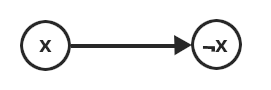
\includegraphics[scale=0.4]{graph_2.png}  \\
leads to clause $x \rightarrow \neg x \equiv \neg x \lor \neg x \equiv \neg x$
\end{itemize}

\item path from $\neg x$ to $x$
\begin{itemize}
\item transitivity of implication
\item[] 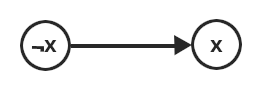
\includegraphics[scale=0.4]{graph_1.png}  \\
leads to clause $\neg x \rightarrow x \equiv \neg \neg x \lor x \equiv x \lor x \equiv x$
\end{itemize}

\item the two clauses are connected with an logic and (because formula is in CNF) which leads to $\neg x \land x$ which is unsatisfiable
\\

\item there are no paths from any $x$ to $\neg x$ and back $x$: no edge is changing from true to false or the other way around
\item whenever a node is assigned to a value, all the successors are assigned to the same value and there can be no edge from true to false or from false to true

\end{itemize}







\subsection*{\textsc{2Sat} in NL}

\textsc{2Sat} is in NL.

\ \\
\textbf{Proof idea:}
\begin{itemize}
\item NL is closed under complement
\item show: unsatisfiable expressions can be recognized in NL
\item nondeterministically guessing a variable $x$ and check for paths between $x$ and $\neg x$ and back
\end{itemize}


\subsection*{\textsc{MaxSat} is NP-complete}

\begin{CountingDefinition}[\textsc{Max2Sat}]{def:validLabelPlacement}
\textsc{Max2Sat} is the problem of determining the maximum number of clauses, of a given Boolean formula in CNF with a maximum of 2 variables per clause, that can be made true by an assignment of truth values to the variables of the formula. 

\textsc{Max2Sat} is an optimization problem.
\end{CountingDefinition}

\textsc{Max2Sat} is NP-complete.

\ \\
\textbf{Example:}
\begin{center}
$(x)(y)(z)(w)$\\
$(\neg x \lor \neg y)(\neg y \lor \neg z)(\neg z \lor \neg x)$ \\
$(x \lor \neg w)(y \lor \neg w)(z \lor \neg w)$
\end{center}

\begin{itemize}
\item not all clauses can be satisfied
\end{itemize}

\ \\
\textbf{Proof idea:}
\begin{itemize}
\item any truth assignment that satisfies $x \lor y \lor z$ satisfies 6 or 7 clauses
\item the remaining truth assignments ($\neg x \land \neg y \land \neg z$) satisfy 4 or 6 clauses
\item reduction from \textsc{3Sat} to \textsc{MaxSat} because $x \lor y \lor z$ needs to be satisfied
\item instance $\psi$ of \textsc{3Sat}
\item instance $R(\psi)$ of \textsc{MaxSat}
\item group clauses of $R(\psi)$ which are corresponding to a clause of $\psi$
\item set constraint of 7 satisfied clauses
\end{itemize}

\color{red} TODO \\
proof \\
\color{black}
\color{violet} Questions:
\color{black}


\subsection*{\textsc{NaeSat} is NP-complete}

\begin{CountingDefinition}[\textsc{NaeSat}]{def:validLabelPlacement}
Like \textsc{SAT}, \textsc{NaeSat} consists of a collection of Boolean variables and clauses. \textsc{NaeSat} requires that the values in each clause are not all equal to each other (in other words, at least one is true, and at least one is false). \cite{moore}
\end{CountingDefinition}

\color{red} TODO \\
\color{black}
\color{violet} Questions:
\color{black}



\newpage

\printbibliography




\end{document}